\section{ХОД РАБОТЫ}

\subsection{Построение мультипликативной модели}

Приведем порядок построения прогноза спроса на товар с использованием
мультипликативной модели.

\begin{enumerate}
\item Вычислим скользящие средние за каждые 4 квартала.
  Расчет выполняется по формуле
  \( \hat{x} = \dfrac{1}{4} (x_{i} + x_{i+1} + x_{i+2} + x_{i+3}) \),
  где \( i \) --- номер начального периода.

  Например, значение скользящего среднего за четыре квартала
  2013 года составляет \( \dfrac{1}{4} (24 + 28 + 27 + 19) = 24{,}5 \),
  а за период со второго квартала 2013 по первый период 2014 года
  включительно --- \( \dfrac{1}{4} (28 + 27 + 19 + 27) = 25{,}25 \).

\item Выполним центрирование полученных значений скользящего среднего
  для того, чтобы их можно было соотнести с конкретными периодами.

  Например, значение скользящего среднего, полученное за четыре квартала
  2013 года, можно отнести как ко второму, так и к третьему кварталу,
  поэтому вычислить среднее между этим и следующим значением:
  \( \dfrac{1}{2} (24{,}5 + 25{,}25) \approx 24{,}88 \) и поставить его
  в соответствие третьему кварталу 2013 года.

\item Вычислим коэффициенты сезонности,
  разделив фактические значения спроса на центрированные скользящие средние.

  Например, определим коэффициенты сезонности за третий квартал
  2013, 2014, 2015 года соответственно:
  \( \dfrac{27}{24{,}88} \approx 1{,}08 \),
  \( \dfrac{29}{28{,}13} \approx 1{,}03 \),
  \( \dfrac{29}{28} \approx 1{,}03 \).
  Значение коэффициента сезонности, большее 1, свидельствует о том, что
  фактическое значение спроса в данном квартале было больше,
  чем усредненное значение.
  Значение коэффициента сезонности, меньшее 1, свидельствует о том, что
  фактическое значение спроса в данном квартале было меньше,
  чем усредненное значение.

\item Вычислим уточненные коэффициенты сезонности путем усреднения
  рассчитанных ранее коэффициентов сезонности,
  сгруппированных по номеру квартала.

  Например,
  значение уточненного коэффициента сезонности для третьего квартала
  составляет
  \( \dfrac{1}{3} (1{,}08 + 1{,}03 + 1{,}03) \approx 1{,}05 \).
  Поставим в соответствие
  вычисленные уточненные коэффициенты сезонности всем сезонам,
  в том числе и тем, спрос на которые должен быть спрогнозирован.

\item Вычислим значения спроса без учета сезонности.
  Для этого выполним деление значений фактического спроса на
  значения уточненных коэффициентов сезонности.

  Например, для третьего квартала 2013 года значение спроса
  без учета сезонности составит \( \dfrac{27}{1{,}05} \approx 25{,}73 \),
  а для третьего квартала 2014 года ---
  \( \dfrac{29}{1{,}05} \approx 27{,}64 \).

\item С помощью метода наименьших квадратов рассчитаем коэффициенты
  линейной функции \( y = A_0 x + A_1 \), аппроксимирующей значения спроса
  без учета сезонности. Расчет удобно выполнять с использованием инструмента
  <<Диаграмма>>, встроенного в табличный процессор Microsoft Excel,
  как показано на рисунке~\ref{fig:mult_without_season}.

  \begin{figure}[h!]
    \centering
    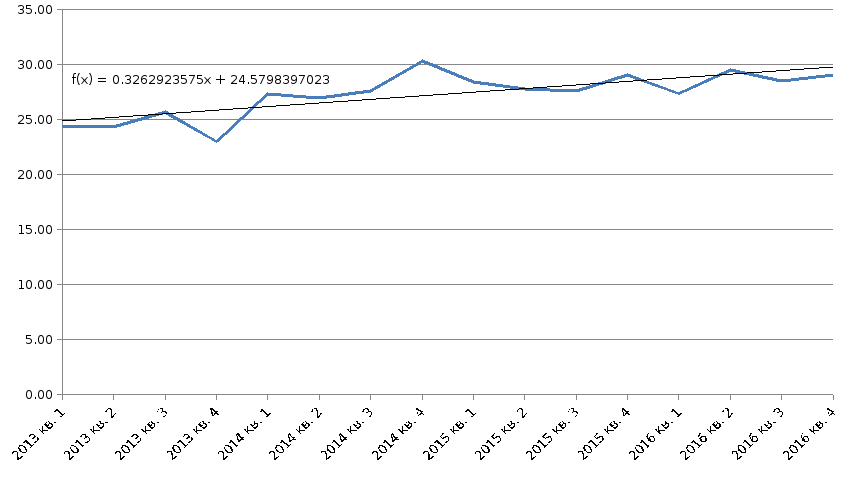
\includegraphics[width=150mm]{pic/mult_without_season}
    \caption{Изменение анализируемой величины во времени \\
      при исключении влияния сезонности (для мультипликативной модели)}
    \label{fig:mult_without_season}
  \end{figure}

  Для нашего случая имеем \( A_0 \approx 0{,}33, A_1 \approx 24{,}58 \).

\item Рассчитаем прогнозируемые значения спроса по формуле
  \( \hat{x} = (A_0 x + A_1) K_c \), где
  \( A_0, A_1 \) --- коэффициенты линейной аппроксимирующей функции,
  рассчитанные ранее,
  \( x = \overline{1,20} \) --- порядковый номер периода,
  \( K_c \) --- уточненный коэффициент сезонности, соответствующий
  данному кварталу.

  Например, для третьего квартала 2013 года модельная величина спроса
  составляет
  \( ( 0{,}33 \cdot 3 + 24{,}58 ) \cdot 1{,}05 \approx 26{,}82 \),
  а для третьего квартала 2017 года ---
  \( ( 0{,}33 \cdot 19 + 24{,}58 ) \cdot 1{,}05 \approx 32{,}29 \).

\item Для оценки точности прогноза, полученного данным методом, вычислим
  среднее значение отклонения прогнозируемых значений от фактических,
  рассчитываемого по формуле
  \begin{equation}
    \label{eq:mad}
    MAD = \dfrac{\sum^n_{i = 1} |x - \hat{x}|}{n},
  \end{equation}
  \hspace{1.5mm} где \( n \) --- число периодов,
  для которых известны и фактические, и прогнозируемые значения спроса.

  Для нашего случая значение \( MAD \) составило 0{,}9.
\end{enumerate}

Проведя указанные вычисления, получим следующие прогнозируемые значения
спроса в 2017 году:

\begin{itemize}
\item первый квартал --- 29{,}67;
\item второй квартал --- 35;
\item третий квартал --- 32{,}29;
\item четвертый квартал --- 25{,}63.
\end{itemize}

Полные результаты прогнозирования с использованием мультипликативной
модели спроса расположены в приложении А.


\subsection{Построение аддитивной модели}

Приведем порядок построения прогноза спроса на товар с использованием
аддитивной модели.

\begin{enumerate}
\item Вычислим скользящие средние за каждые 4 квартала.
  Расчет выполняется по формуле
  \( \hat{x} = \dfrac{1}{4} (x_{i} + x_{i+1} + x_{i+2} + x_{i+3}) \),
  где \( i \) --- номер начального периода.

  Например, значение скользящего среднего за четыре квартала
  2013 года составляет \( \dfrac{1}{4} (24 + 28 + 27 + 19) = 24{,}5 \),
  а за период со второго квартала 2013 по первый период 2014 года
  включительно --- \( \dfrac{1}{4} (28 + 27 + 19 + 27) = 25{,}25 \).

\item Выполним центрирование полученных значений скользящего среднего
  для того, чтобы их можно было соотнести с конкретными периодами.

  Например, значение скользящего среднего, полученное за четыре квартала
  2013 года, можно отнести как ко второму, так и к третьему кварталу,
  поэтому вычислить среднее между этим и следующим значением:
  \( \dfrac{1}{2} (24{,}5 + 25{,}25) \approx 24{,}88 \) и поставить его
  в соответствие третьему кварталу 2013 года.

\item Вычислим компоненты сезонности,
  вычтя центрированные скользящие средние значения спроса из фактических.

  Например, определим компоненты сезонности за третий квартал
  2013, 2014, 2015 года соответственно:
  \( 27 - 24{,}88 \approx 2{,}13 \),
  \( 29 - 28{,}13 \approx 0{,}88 \),
  \( 29 - 28{,}13 \approx 0{,}88 \).
  Значение компоненты сезонности, большее 0, свидельствует о том, что
  фактическое значение спроса в данном квартале было больше,
  чем усредненное значение.
  Значение компоненты сезонности, меньшее 0, свидельствует о том, что
  фактическое значение спроса в данном квартале было меньше,
  чем усредненное значение.

\item Вычислим уточненные компоненты сезонности путем усреднения
  рассчитанных ранее компонент сезонности,
  сгруппированных по номеру квартала.

  Например,
  значение уточненной компоненты сезонности для третьего квартала составляет
  \( \dfrac{1}{3} (2{,}13 + 0{,}88 + 0{,}88) \approx 1{,}29 \).
  Поставим в соответствие
  вычисленные уточненные коэффициенты сезонности всем сезонам,
  в том числе и тем,
  спрос на которые должен быть спрогнозирован.

\item Вычислим значения спроса без учета сезонности.
  Для этого выполним вычитание значений уточненных компонент сезонности из
  значений фактического спроса.

  Например, для третьего квартала 2013 года значение спроса
  без учета сезонности составит \( 27 - 1{,}29 = 25{,}71 \),
  а для третьего квартала 2014 года ---
  \( 29 - 1{,}29 = 27{,}71 \).

\item С помощью метода наименьших квадратов рассчитаем коэффициенты
  линейной функции \( y = A_0 x + A_1 \), аппроксимирующей значения спроса
  без учета сезонности. Расчет удобно выполнять с использованием инструмента
  <<Диаграмма>>, встроенного в табличный процессор Microsoft Excel,
  как показано на рисунке~\ref{fig:add_without_season}.

  \begin{figure}[h!]
    \centering
    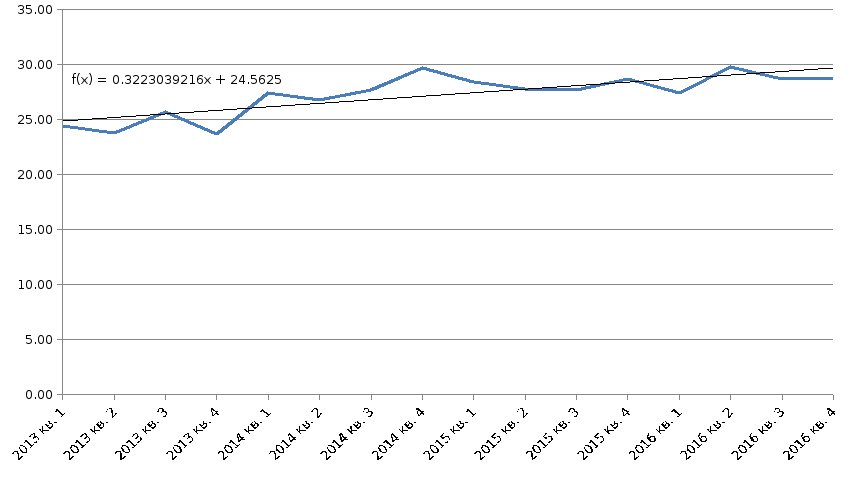
\includegraphics[width=150mm]{pic/add_without_season}
    \caption{Изменение анализируемой величины во времени \\
      при исключении влияния сезонности (для аддитивной модели)}
    \label{fig:add_without_season}
  \end{figure}

  Для нашего случая имеем \( A_0 \approx 0{,}32, A_1 \approx 24{,}56 \).

\item Рассчитаем прогнозируемые значения спроса по формуле
  \( \hat{x} = (A_0 x + A_1) + K_c \), где
  \( A_0, A_1 \) --- коэффициенты линейной аппроксимирующей функции,
  рассчитанные ранее,
  \( x = \overline{1,20} \) --- порядковый номер периода,
  \( K_c \) --- уточненная компонента сезонности, соответствующая
  данному кварталу.

  Например, для третьего квартала 2013 года модельная величина спроса
  составляет
  \( ( 0{,}32 \cdot 3 + 24{,}56 ) + 1{,}29 \approx 26{,}82 \),
  а для третьего квартала 2017 года ---
  \( ( 0{,}32 \cdot 19 + 24{,}56 ) + 1{,}29 \approx 31{,}98 \).

\item Для оценки точности прогноза, полученного данным методом, вычислим
  среднее значение отклонения прогнозируемых значений от фактических,
  рассчитываемого по формуле~\ref{eq:mad}.

  Для нашего случая значение \( MAD \) составило 0{,}91.
\end{enumerate}

Проведя указанные вычисления, получим следующие прогнозируемые значения
спроса в 2017 году:

\begin{itemize}
\item первый квартал --- 29{,}58;
\item второй квартал --- 34{,}57;
\item третий квартал --- 31{,}98;
\item четвертый квартал --- 26{,}26.
\end{itemize}

Полные результаты прогнозирования с использованием мультипликативной
модели спроса расположены в приложении Б.


\subsection{Сравнение результатов моделирования}

Для определения наиболее точного метода моделирования из рассмотренных
выше сравним значения \( MAD \):
0{,}9 для мультипликативной модели спроса и
0{,}91 --- для аддитивной.
Поскольку \( 0{,}9 < 0{,}91 \), то более точной будем считать мультипликативную модель спроса.

Таким образом, окончательным результатом решения задачи являются следующие
прогнозируемые значения спроса,
полученные с помощью мультипликативной модели:

\begin{itemize}
\item первый квартал 2017 года --- 29{,}67;
\item второй квартал 2017 года --- 35;
\item третий квартал 2017 года --- 32{,}29;
\item четвертый квартал 2017 года --- 25{,}63.
\end{itemize}
